\section{Hash-Mode Results}
\label{sec:hash-results}
The controlled study keeps CQF memory identical across modes: 1,472,416 bytes in the 996,148-operation control and 186,807,707 bytes at 67M. Figure~\ref{fig:hash-speedup} expresses each mean rate relative to the default path at the same scale and distribution. Ratios compare means; the accompanying raw tables retain the three individual runs.

\begin{figure}[!htbp]\centering
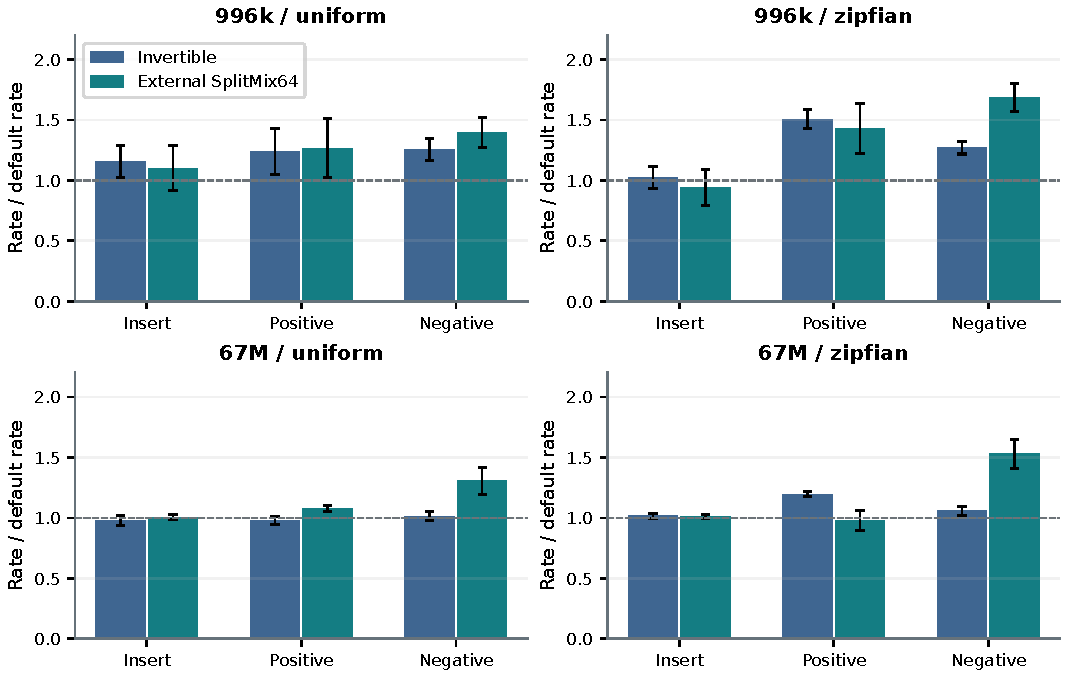
\includegraphics[width=\linewidth]{hash_speedups.pdf}
\caption{End-to-end CQF rate relative to default MurmurHash ($1\times$). The 996k control uses $q=20$; the 67M study uses $q=27$. Insertions and both query classes include the corresponding hash cost. Error bars show an approximate propagated descriptive SD, assuming independent run noise; they are not confidence intervals for the ratios.}
\label{fig:hash-speedup}
\end{figure}

At 67M uniform input, external SplitMix64 changes the negative-query rate from \HashDefaultNegativeUniform{} to \HashExternalNegativeUniform{}\Mops{}, a ratio of \HashExternalNegativeUniformRatio{}$\times$. Its uniform insertion ratio is \HashExternalInsertUniformRatio{}$\times$. On skewed input, its negative-query ratio is \HashExternalNegativeSkewRatio{}$\times$, while its insertion ratio is \HashExternalInsertSkewRatio{}$\times$. These differences show why we do not describe one mode as an unconditional improvement for every operation.

\begin{table}[!htbp]\centering\small
\caption{67M hash-path accuracy, first repetition with 10M negatives. The estimate uses the distinct original-key count over the configured fingerprint domain. Invertible mode retains a non-zero collision probability for these wider input keys.}
\label{tab:hash-accuracy}
\begin{tabular}{@{}llrrr@{}}
\toprule
\textbf{Input} & \textbf{Path} & \textbf{Measured} & \textbf{95\% interval} & \textbf{Estimate} \\
\midrule
Uniform & Default & $9.69\times10^{-4}$ & [$9.50\times10^{-4}$, $9.89\times10^{-4}$] & $9.75\times10^{-4}$ \\
Uniform & Invertible & $9.66\times10^{-4}$ & [$9.47\times10^{-4}$, $9.86\times10^{-4}$] & $9.75\times10^{-4}$ \\
Uniform & External & $9.79\times10^{-4}$ & [$9.60\times10^{-4}$, $9.98\times10^{-4}$] & $9.75\times10^{-4}$ \\
Zipfian & Default & $2.50\times10^{-6}$ & [$1.69\times10^{-6}$, $3.69\times10^{-6}$] & $3.33\times10^{-6}$ \\
Zipfian & Invertible & $3.70\times10^{-6}$ & [$2.68\times10^{-6}$, $5.10\times10^{-6}$] & $3.33\times10^{-6}$ \\
Zipfian & External & $3.50\times10^{-6}$ & [$2.52\times10^{-6}$, $4.87\times10^{-6}$] & $3.33\times10^{-6}$ \\
\bottomrule
\end{tabular}

\end{table}

The hash choices do not change the CQF's counter representation or memory allocation. Their FPR estimates are consequently the same within a workload, while the measured samples differ with the mapping. At the skewed 67M operating point, the expected number of false positives is only about 33 in 10M queries, so rate ratios can look large even when the absolute difference is a few queries. Neither the lowest observed rate nor the fastest one-operation result is enough to nominate a universally best mixer.

The most defensible practical outcome is to expose the hash choice, measure the operation mix that matters, and verify positive recognition and accuracy after changing it. We retain the default path for the primary seven-filter comparison to avoid mixing a hash substitution with the filter-family comparison.
\clearpage
